\section{Current Testing Strategy and its Flaws}

So called "KeTops" are used as operating devices to control machines of varying structure and complexity. These machines and their corresponding KeTops differ in their configuration from each customer which is why fitting test scripts are required. These test scripts examine all aspects of the device from the installed operating system to software specific behaviors. 

The \textit{Script Assembler} which is used in current production is able to merge a number of test scripts together for this use. The hard-coded nature and resulting limited maintainibility of the Script Assembler is its primary flaw. Furthermore all data concerning tests are saved and maintained in a TestRail database which although functional, heavily limits the expandability and independence of the testing environment.

\section{Acceptance Tests}

The Robot Framework is a test automation framework designed to create and execute the test scripts in the current system. These tests are acceptance tests, which are a type of test that is created before the actual implementation of the software. The purpose of acceptance tests is to define the expected behavior of the system from the perspective of the customer or end-user. They serve as a guide to ensure that the development team is building the software according to the expectations of said customer \cite{WikiRobotFramework}.

Acceptance tests typically consist of terms understandable by both technical and non-technical parties, making them understandable regardless of the expertise of the reader. They intend to cover all the requirements and functionalities of the system and serve as a list of criteria for acceptance \cite{WikiAcceptanceTestDrivenDev}.

\subsection{Different Types of Tests and the V-Model}

The V-Model emphasizes the importance of consistent testing throughout the development process of software. In the first half of the V-Model, the focus is on defining the concept of the system as a whole and its requirements. Further on, the definition is broken down into smaller and smaller components, until we reach the detailed design of the software. Afterwards, the implementation takes place, which is the point where the actual code is written.

The second half of the V-Model focuses on testing each corresponding unit on the same level of the first half. During each design phase, a corresponding set of tests is created, which are responsible for testing the software at that level.

For example, during the module design phase, unit tests are created, which are responsible for testing the code at its most basic level, ensuring the system functions without bugs or errors \cite{WikiVModel}.

The V-Model displays the design and testing phases in a V shape, as seen in figure \ref{fig:v-model}.

\begin{figure}[h]
    \centering
    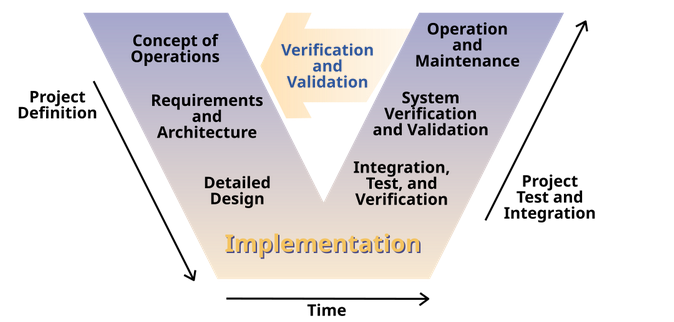
\includegraphics[width=0.5\textwidth]{pics/v-model.png}
    \caption{V-Model of software development and testing \cite{WikiVModel}}
    \label{fig:v-model}
\end{figure}

\section{Goals and Objectives}

This project aims to eliminate all of the listed problems and concerns while building upon and improving the existing capabilites of the Script Assembler. 

\begin{itemize}
    \item \textbf{EBNF parsing:} \\
    The existing structure of the test scripts should be formed into its own EBNF language which is then integrated into the Script Assembler. This eliminates a majority of the hard-coded parts of the software. Furthermore the editor should provide appropriate syntax highlighting when writing or editing a test script.

    \item \textbf{Keyword support:} \\
    New functionalities should be implemented which allows the editor of test scripts to specify aspects like the version and the operating system the test has to be run on. The structure of keywords need to be precisely set in the EBNF language.

    \item \textbf{Database mock:} \\
    The structure of the currently used TestRail database should be studied and an accurate mockup should be created. A seamless switch between the mock and the real TestRail instance has to be implemented as well.
\end{itemize}